
\documentclass[12pt]{report}
\usepackage[utf8]{inputenc}
\usepackage[english]{babel}
\usepackage{hyphenat}
\usepackage{graphicx}
\usepackage{amsmath}
\usepackage[colorlinks=true, linkcolor=blue, citecolor=blue, urlcolor=blue]{hyperref}
\usepackage{geometry}
\usepackage{fancyhdr}
\setlength{\headheight}{15pt}
\usepackage{setspace}
\usepackage{csquotes}
\usepackage{float}
\usepackage[colorinlistoftodos,prependcaption,textsize=small]{todonotes}

\usepackage[backend=biber,style=apa]{biblatex}
\addbibresource{references.bib}


\documentclass[11pt,a4paper]{article}
\usepackage[T1]{fontenc}
\usepackage{titlesec}

% ===========================
% Layout according to IU specs
% ===========================
\geometry{a4paper, top=2cm, bottom=2cm, left=2cm, right=2cm}
\setstretch{1.5} % Line spacing

% Font sizes: 11pt text, 12pt headings
\renewcommand\normalsize{\fontsize{11}{13.6}\selectfont}
\renewcommand\footnotesize{\fontsize{10}{12}\selectfont}

% Paragraphs: 6pt spacing after, no indent
\setlength{\parskip}{6pt}
\setlength{\parindent}{0pt}

% Numbering: max. 3 levels
\setcounter{secnumdepth}{3}

% Heading formatting
\titleformat{\section}{\fontsize{12}{14}\bfseries}{\thesection}{1em}{}
\titleformat{\subsection}{\fontsize{12}{14}\bfseries}{\thesubsection}{1em}{}
\titleformat{\subsubsection}{\fontsize{12}{14}\itshape}{\thesubsubsection}{1em}{}

% ===========================
% Title Page
% ===========================
\begin{document}
\begin{titlepage}
    \centering

    {\LARGE Master's Aptitude Thesis\par}
    \vspace{0.5cm}
    {\Large AI-Driven Impact Measurement and Management: \par
    Design and Evaluation of a Framework using the Inluma Case \par
    under the Design Science Research Methodology \par}
    \vspace{1.5cm}

    {\large Dean Didion \par}
    Matriculation Number: IU14148408 \par
    \vspace{1.5cm}

    Study Program: M.Sc. Applied Artificial Intelligence \par
    Module: Preparation – Master for Professionals \par
    \vfill

    Date: \today
\end{titlepage}


%! Author = deandidion
%! Date = 11.07.25

% Document
\begin{abstract}
Measuring social and economic impact has become increasingly important in public sector innovation, as governments and organizations aim to demonstrate accountability and optimize resource use~\parencite{oecd2020, giin2023}.
The growing number of impact-focused startups and initiatives highlights a broader shift towards mission-driven work that prioritizes measurable public value and sustainable outcomes~\parencite{phineo2023, unternehmertum2023}.

This thesis explores how artificial intelligence (AI) can support impact measurement within this evolving context.
It is situated at the Public Value Hub in Leipzig and contributes to the ongoing development of the Public Value Academy software platform.
The primary goal is to develop a framework for AI-supported impact measurement that balances technical feasibility with alignment to public values.

The work draws on established Impact Measurement and Management (IMM) concepts from Phineo, alongside practical guidance from UnternehmerTUM. These inform both the conceptual foundations and the requirements for a scalable, real-world solution.

Methodologically, the research combines stakeholder interviews with the implementation of AI components in Python.
These components illustrate how intelligent systems can foster transparent, data-driven evaluations in a sector where social outcomes are paramount.

By bridging theory and practice, the thesis demonstrates how AI can responsibly enhance public innovation, promote accountability, and strengthen impact-oriented approaches in the public sector.
\end{abstract}

\tableofcontents
\listoffigures

\newpage

%! Author = Dean Didion
%! Date = 09.07.25

\chapter{Introduction}\label{ch:introduction}


\section{Background}\label{sec:background}

Innovation in the public sector is increasingly seen as essential for tackling complex societal challenges.
As governments and public institutions explore new ways to deliver services, assess policy outcomes, and engage with citizens, the question of \textbf{impact} becomes central.
While private sector innovations often measure success through profit and efficiency, public sector innovation needs to be evaluated against broader societal value, which is a much more nuanced and multidimensional goal.

Artificial Intelligence (AI) has emerged as a powerful tool for analyzing vast datasets, identifying complex patterns, and supporting evidence-based decision-making~\parencite{russell2016artificial, marr2018data}.
In the public sector, AI holds significant promise for enhancing transparency, accountability, and responsiveness.
A recent study (see~\cite{cornell2024}) carried out on UK public service professionals showed that about 22\% actively use generative AI and 45\% are aware of AI tools in their area, it is still \textit{not routinely applied} to assess the impact of innovation initiatives.


\begin{figure}[H]
  \centering
  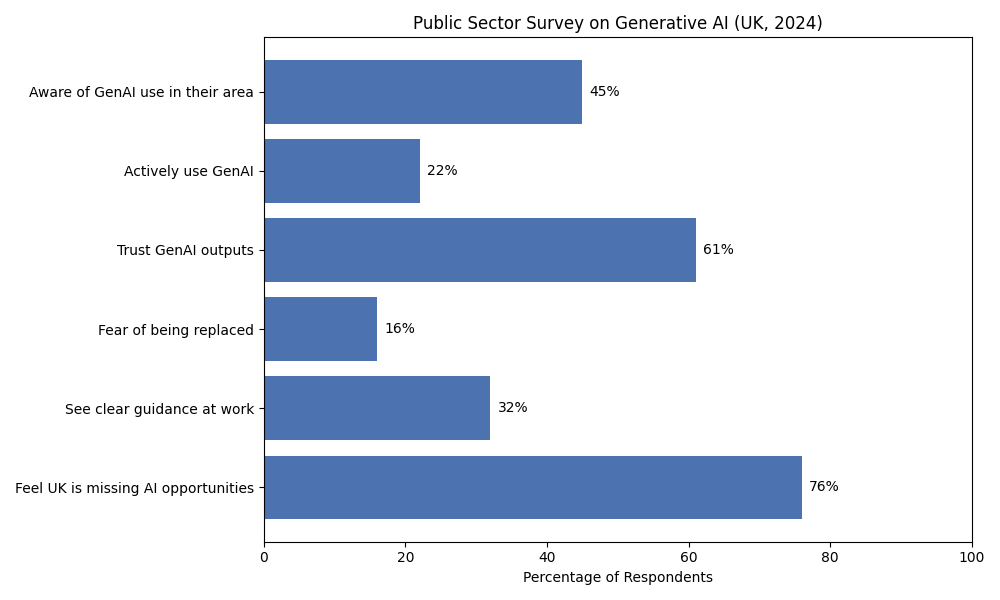
\includegraphics[width=0.8\textwidth]{../fig/ai_awareness_uk}
  \caption{Public sector professionals' attitudes toward generative AI.}
  \label{fig:genai_survey}
  \caption*{\textit{Source:}~\parencite{cornell2024}}
\end{figure}


Traditional impact measurement frameworks—while widely used—are often too rigid for the dynamic and experimental nature of many public sector initiatives (see Figure~\ref{fig:rigid_frameworks})
These frameworks may not accommodate evolving goals, emergent outcomes, or context-specific indicators.
Moreover, despite the variety of available frameworks, organizations tend to rely on a single predefined model, often because it is mandated or institutionally recognized.
This one-size-fits-all approach can limit flexibility and hinder meaningful evaluation.
There is, therefore, a growing need for more adaptive, intelligent systems that can integrate multiple perspectives and evolve alongside the initiatives they aim to assess.

\begin{figure}[H]
  \centering
  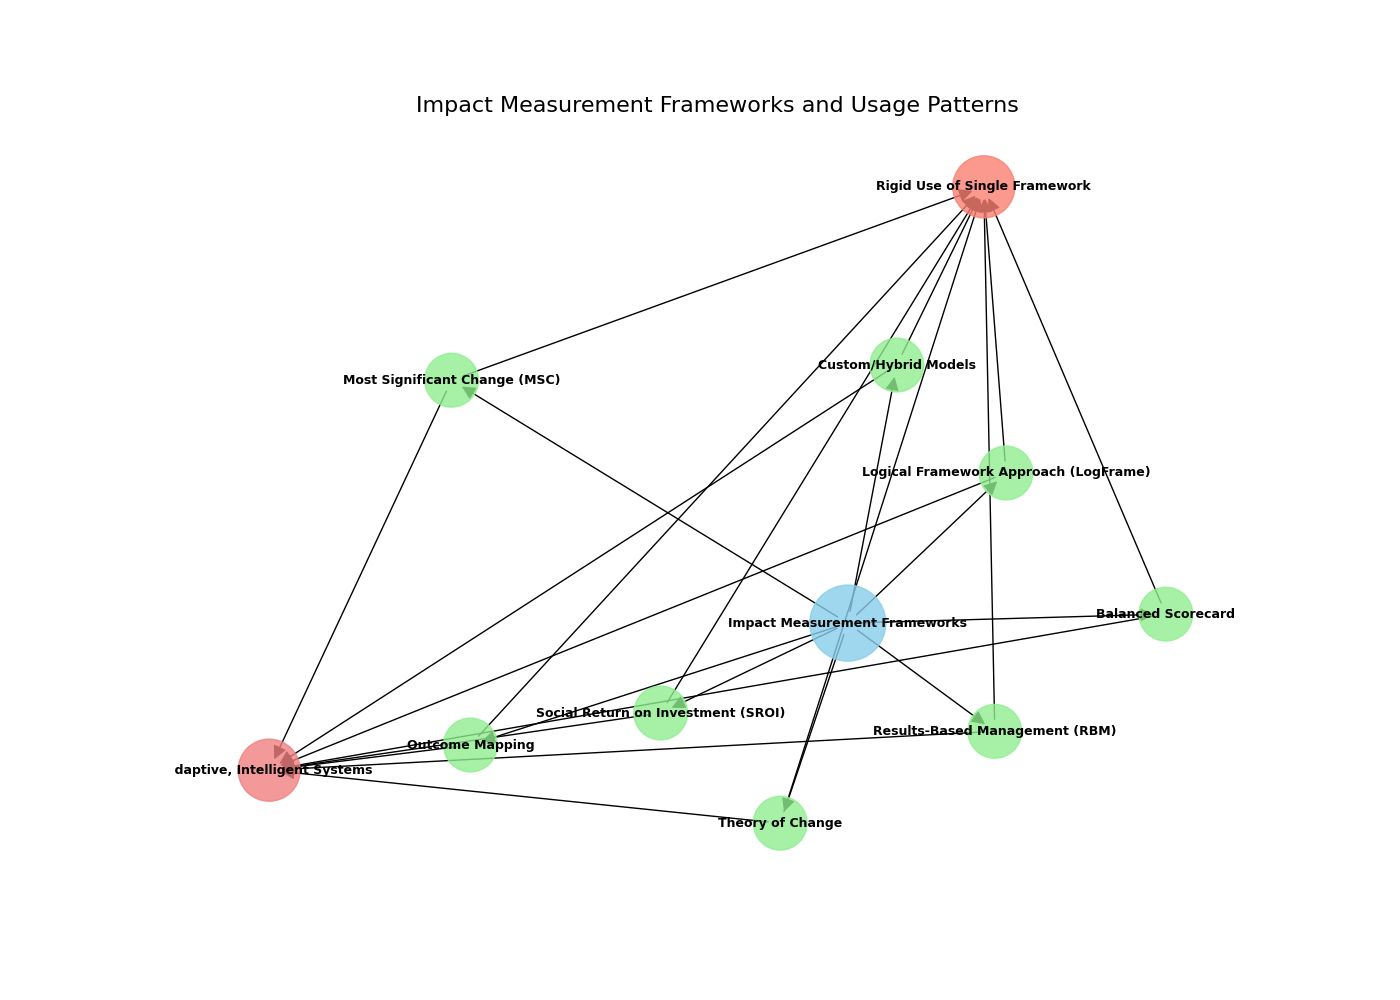
\includegraphics[width=0.8\textwidth]{../fig/rigid_use_frameworks}
  \caption{Rigid use of single frameworks}
  \label{fig:rigid_frameworks}
\end{figure}

This thesis is embedded in a real-world initiative from the \textbf{Public Value Hub in Leipzig} and aligns with the goals of the \textbf{Public Value Academy}, an emerging digital platform aimed at fostering innovation literacy and sustainable impact measurement in the public sector.

\section{Problem Statement}\label{sec:problem-statement}
Despite the growing use of AI across sectors, there remains a significant gap in how AI can support \textbf{meaningful, qualitative impact assessment} — particularly in the public domain.
Existing tools often rely on rigid indicators and retrospective analysis, failing to capture complexity, learning, or long-term public value creation~\parencite{ebrahim2014impact, patton2011developmental}.
Moreover, public sector organizations often lack the resources or knowledge to adopt AI tools effectively~\parencite{mikhaylov2018ai}.
Furthermore, public sector organizations often do not have access to the resources or knowledge to adopt and adapt AI tools effectively.

There is a need to explore \textbf{how AI technologies can be applied to support dynamic, context-sensitive, and participatory impact measurement}, integrating frameworks such as those developed by \textbf{PHINEO} and supported by \textbf{UnternehmerTUM’s educational content}.

\section{Objectives}\label{sec:objectives}
The aim of this thesis is to develop a \textbf{conceptual and technical framework} for AI-supported impact measurement.
By combining theory, stakeholder insights, and prototyping with Python-based methods, the goal is to investigate how such a system could function in practice as part of the Public Value Academy’s software platform.

\section{Research Questions}\label{sec:research-questions}

This thesis investigates the potential of artificial intelligence to enhance impact measurement practices.
Given the complexity and evolving nature of public value creation, the research is guided by the following questions:

\begin{itemize}
  \item \textbf{How can artificial intelligence contribute to improved impact measurement in public sector innovation?} \\
  This question explores the capabilities of AI to support more nuanced, dynamic, and qualitative assessments beyond traditional rigid indicators.

  \item \textbf{What are the challenges and opportunities of integrating AI with existing single frameworks} \\
  Here, the focus is on identifying barriers, enablers, and practical considerations when combining AI tools with established impact measurement methodologies.

  \item \textbf{What would a prototype AI-supported measurement tool look like in practice?} \\
  This question aims to conceptualize and design a practical application that demonstrates how AI can be embedded in impact measurement workflows.
\end{itemize}

\section{Scope and Limitations}\label{sec:scope-and-limitations}

This thesis focuses on the \textbf{conceptual design and development} of an AI-supported measurement framework.
The implementation centers on a \textbf{Python-based Minimum Viable Product (MVP)} that demonstrates core functionalities but stops short of a full-scale deployment.
While informed by existing frameworks and stakeholder input, it does not include extensive empirical validation.

\medskip
\noindent\textbf{Note:} The focus is on \textbf{public innovation projects} in the German context, though the framework has broader applicability.
\medskip

\section{Methodology Overview}\label{sec:methodology-overview}

The research combines:
\begin{itemize}
\item
A literature review on impact measurement and AI in the public sector,
\item
Exploration of frameworks (such as PHINEO’s IMM),
\item
Qualitative insights from relevant stakeholders (e.g. Public Value Hub),
\item
And the development of basic Python-based prototypes to test technical feasibility and application logic.
\end{itemize}

\section{Structure of the Thesis}\label{sec:structure-of-the-thesis}

This thesis is structured as follows:

\begin{itemize}
\item
\textbf{Chapter 2} presents the theoretical and conceptual background, including relevant literature on AI, impact measurement, and public value.
\item
\textbf{Chapter 3} outlines the methodology and design process used in this research.
\item
\textbf{Chapter 4} presents the key findings from prototype development and stakeholder insights.
\item
\textbf{Chapter 5} discusses the results in the context of existing frameworks and reflects on challenges and opportunities.
\item
\textbf{Chapter 6} concludes the thesis with a summary of key insights and recommendations for further development.
\end{itemize}

\chapter{Theoretical Background}\label{ch:theoretical-background}

\section{Introduction}\label{sec:introduction}
This chapter reviews existing literature across three interconnected areas: \textbf{Impact Measurement and Management (IMM)}, \textbf{public sector innovation (PSI)}, and the application of \textbf{Artificial Intelligence (AI)} in these domains.
The objective is to establish a conceptual foundation for AI-supported, values-driven impact evaluation in public innovation ecosystems, and to identify gaps that the thesis artefact implemented in \textit{Inluma} will address.

\section{Impact Measurement and Management (IMM)}\label{sec:imm}
The measurement of impact, particularly in social and public sector contexts, has evolved significantly over the past decades.
Scholars such as \textcite{ebrahim2014measuring} emphasize the importance of aligning measurement approaches with a theory of change and organizational strategy.
Organizations often struggle to balance accountability and learning, particularly when the expected impact is diffuse or long-term.

\textcite{nicholls2012measuring} highlight tensions between standardized, quantitative measurement systems and the qualitative, context-specific nature of many social interventions.
Their work formalizes a typology of impact logic models, demonstrating that one-size-fits-all approaches are rarely effective.

In the German context, intermediaries such as Phineo and UnternehmerTUM provide practical IMM frameworks tailored to social enterprises and innovation labs.
These frameworks integrate stakeholder mapping, output-outcome mapping, and logic modelling to clarify how public interventions generate value.

\begin{figure}[H]
    \centering
    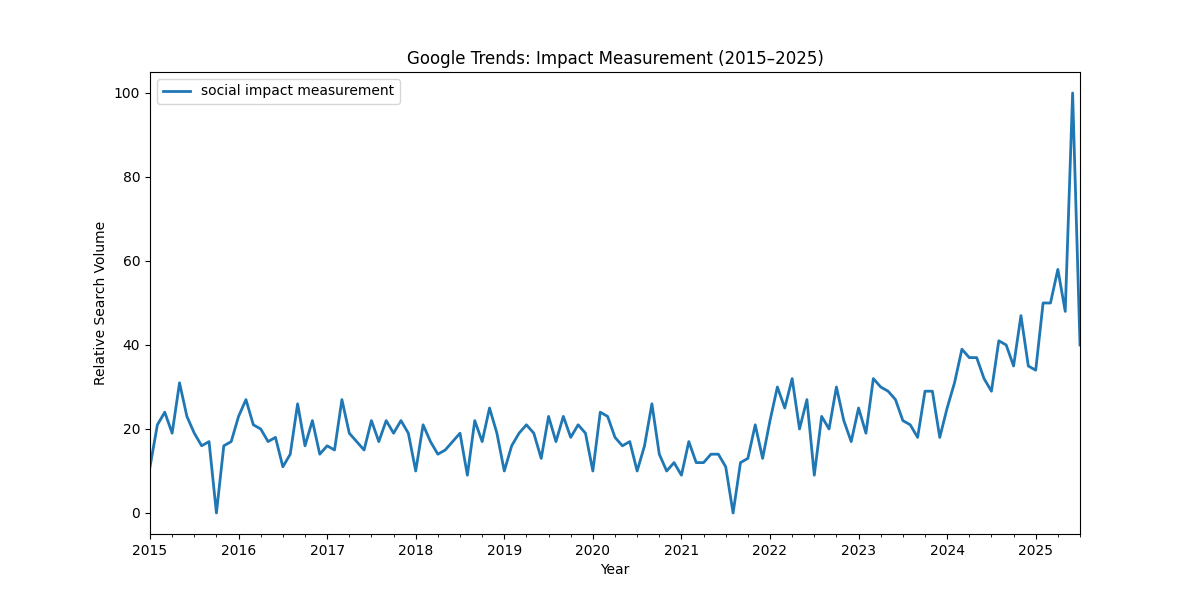
\includegraphics[width = 0.8\textwidth]{../fig/google_trend_impact}
    \caption{Google trend for "impact measurement".}
    \label{fig:trend_impact}
\end{figure}

\section{Public Sector Innovation and Value Creation}\label{sec:public-sector-innovation}
Public sector innovation requires institutions to not only introduce new tools or practices but also foster legitimacy, collaboration, and accountability~\parencite{sun2019algorithmic}.
The OECD has documented challenges and opportunities associated with innovation in government, including an increasing emphasis on public value creation, citizen co-production, and agile experimentation~\parencite{oecd2020publicsector}.

\textcite{wirtz2020public} propose a conceptual model for digital transformation in public services, emphasizing that data-driven approaches can enhance or erode trust depending on their transparency, inclusiveness, and fairness.
The concept of \textbf{public value}—first introduced by Moore (1995) and later expanded—serves as a central reference for evaluating the outcomes of public innovation.
Initiatives such as Project Athena and CityLAB Berlin exemplify stakeholder-driven innovation aligned with public value frameworks.

\section{Artificial Intelligence Methods for Qualitative and Quantitative Data Analysis}\label{sec:ai-methods}
AI has become increasingly prevalent in public governance, ranging from algorithmic decision-making to NLP-based policy analysis.
\textcite{devlin2018bert} introduced BERT, a transformer-based model foundational for text classification, topic modeling, and semantic similarity analysis.
Such methods can be applied to IMM to analyze unstructured stakeholder data, such as survey responses or social media feedback.

\textcite{sun2019algorithmic} caution that AI must be embedded within deliberative governance structures to ensure its use complements rather than replaces human judgment.
Similarly, \textcite{brown2020algorithmic} highlight that while AI can improve monitoring and accountability, it carries risks such as value misalignment, opacity, and exclusion.
In this thesis, AI is employed within the IMM tool \textit{Inluma} to augment human interpretation, particularly in the analysis of complex qualitative narratives.

\section{Synthesis and Gaps}\label{sec:synthesis-gaps}
IMM frameworks, public sector innovation, and AI-supported decision-making offer complementary approaches to tackle complex societal challenges.
However, an integrated framework that unifies these domains is largely absent.
Traditional IMM approaches often rely on structured metrics and overlook unstructured qualitative data~\parencite{epstein_yuthas_2014,fraunhofer_2023}.
Public sector innovation initiatives emphasize stakeholder engagement and legitimacy but underutilize AI to scale qualitative data analysis~\parencite{citylab_2024}.
AI applications, while powerful, often prioritize efficiency over social complexity and normative commitments such as transparency, equity, and public value~\parencite{moore_1995,benington_moore_2011,eu_2024}.

This thesis addresses these gaps by proposing a framework where AI in \textit{Inluma} augments human interpretation, integrates stakeholder input, and aligns with public value principles.
For example, a Hamburg municipality's digital inclusion initiative could be analyzed using NLP tools to identify barriers like affordability, with stakeholders validating results and refining impact metrics.
This framework bridges IMM’s technical limitations and AI’s normative shortcomings, offering an inclusive, transparent, and effective approach to public sector impact measurement.

\begin{figure}[H]
    \centering
    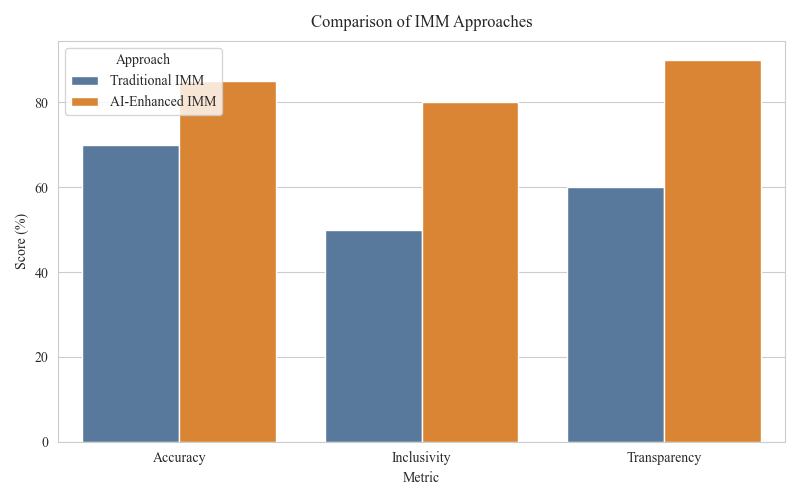
\includegraphics[width=0.8\linewidth]{../fig/imm_comparison}
    \caption{Comparison of IMM frameworks.}
    \label{fig:comparison_imm_fw}
\end{figure}

\section{Conclusion and Research Direction}\label{sec:conclusion}
This chapter has established the theoretical foundation for the thesis, integrating literature on IMM, AI methods, and public sector innovation.
It highlights the research gap that motivates the design, implementation, and evaluation of an AI-supported IMM artefact in \textit{Inluma}.
The following chapter presents the methodology used to develop and assess this framework.

\chapter{Methodology}\label{ch:methodology}

This chapter outlines the methodology guiding this research.
Building on the principles of \textbf{Design Science Research (DSR)}, it describes the process through which an AI-enabled Impact Measurement and Management (IMM) artefact was designed, developed, demonstrated, and evaluated within the context of \textit{Inluma} and the Public Value Hub in Leipzig.
The chapter first introduces the methodological foundation, then explains the research context, followed by the stages of artefact creation and evaluation, and concludes with reflections on contributions and ethical considerations.

% ===========================
% SECTION 3.1
% ===========================
\section{Research Methodology}\label{sec:research-methodology}

This research applies the \textbf{Design Science Research (DSR)} methodology, which provides a structured process for developing and evaluating innovative artefacts in information systems research~\parencite{hevner2004design, peffers2007design}.
DSR is particularly suited to this thesis, as the objective is not only to analyze existing IMM practices but to design, implement, and evaluate a novel artefact that integrates Artificial Intelligence (AI) into impact measurement and management.

The artefact is implemented as a \textbf{prototypical instantiation}—a proof of concept designed to explore feasibility and generate insights for future development.
The evaluation therefore focuses on usability, interpretability, and improvement potential rather than generalizability or market readiness.

Following the DSR framework, the research proceeds through six iterative stages (Figure~\ref{fig:dsr-cycle}): problem identification, knowledge base grounding, artefact design and development, demonstration, evaluation, and reflection and contribution.

% ===========================
% DSR process cycle figure
% ===========================
\begin{figure}[h!]
    \centering
    \begin{tikzpicture}[
        node distance=2.5cm,
        every node/.style={font=\sffamily, align=center},
        box/.style={rectangle, rounded corners, draw=black, fill=gray!10, minimum width=3.8cm, minimum height=1cm},
        arrow/.style={-{Stealth[length=3mm,width=2mm]}, thick}
    ]

    % Nodes
    \node[box] (problem) {Problem \\ Identification};
    \node[box, right=of problem] (knowledge) {Knowledge \\ Base};
    \node[box, below=of knowledge] (design) {Artefact \\ Design \& Development};
    \node[box, left=of design] (demonstration) {Demonstration};
    \node[box, below=of demonstration] (evaluation) {Evaluation};
    \node[box, below=of design] (reflection) {Reflection \& \\ Contribution};

    % Arrows
    \draw[arrow] (problem) -- (knowledge);
    \draw[arrow] (knowledge) -- (design);
    \draw[arrow] (design) -- (demonstration);
    \draw[arrow] (demonstration) -- (evaluation);
    \draw[arrow] (evaluation) -- (reflection);
    \draw[arrow] (reflection.west) .. controls +(-2,0) and +(-2,0) .. (problem.west);

    \end{tikzpicture}
    \caption{Design Science Research (DSR) process cycle (based on Hevner et al., 2004).}
    \label{fig:dsr-cycle}
\end{figure}


% ===========================
% SECTION 3.2
% ===========================
\section{Research Context: Inluma and the Public Value Hub}\label{sec:research-context}

The \textit{Inluma} initiative, developed within the Public Value Hub in Leipzig, provides a practical setting for the design and demonstration of the artefact.
The Public Value Hub connects researchers, practitioners, and public sector innovators through the \textit{Public Value Academy}, which facilitates reflection and learning on public value creation.
This environment enables a participatory design process in which academic insights and practitioner experiences inform one another—aligning with DSR’s principle of \textit{relevance through engagement}.

\textit{Inluma} functions as both a conceptual framework and a digital platform for exploring AI-supported learning and reflection processes.
It is therefore well suited for the iterative development and evaluation of a proof-of-concept artefact within a real-world innovation ecosystem.


% ===========================
% SECTION 3.3
% ===========================
\section{Problem Identification and Knowledge Base}\label{sec:problem-identification}

The first stages of the DSR process involve identifying the practical problem and grounding it in a solid theoretical and empirical knowledge base.
In this research, qualitative inquiry was employed to understand existing challenges in impact measurement and management and to identify opportunities for AI integration.

Semi-structured interviews and participatory workshops were conducted with public sector innovators and researchers affiliated with the Public Value Hub and the Public Value Academy.
These engagements focused on:
\begin{itemize}
    \item Limitations in current impact measurement and reporting practices,
    \item Approaches to operationalizing concepts such as \textbf{public value} and \textbf{social impact},
    \item Stakeholder needs for learning, reflection, and transparency in evaluation processes.
\end{itemize}

A thematic analysis of the qualitative data informed the artefact’s design requirements.
Key insights emphasized the need for interpretability, adaptability, and the ability to integrate both quantitative and narrative dimensions of impact.
The theoretical grounding draws on literature from impact measurement, artificial intelligence, and public sector innovation, providing the knowledge base that guides artefact development.


% ===========================
% SECTION 3.4
% ===========================
\section{Artefact Design and Development}\label{sec:artefact-design}

The central outcome of the DSR process is the design and development of an artefact that addresses the identified problem.
In this case, the artefact is an \textbf{AI-enabled Impact Measurement and Management (IMM) framework} instantiated within the \textit{Inluma} environment.
It aims to support sense-making in impact assessment through natural language processing (NLP), semantic search, and automated knowledge organization.

The artefact consists of four interconnected modules:

\subsection{Narrative Analysis of Pitch Decks}
This module uses large language models (LLMs) to analyze qualitative project materials such as pitch decks or reports.
It extracts key entities, identifies value propositions, and translates narrative inputs into structured representations.

\subsection{Semantic Similarity Search Across Frameworks}
An embedding-based search mechanism allows comparison between project narratives and reference frameworks such as the Sustainable Development Goals (SDGs) or public value dimensions.
This enables contextual mapping of activities and outcomes.

\subsection{Clustering and Thematic Grouping of Narratives}
Using vector embeddings, thematically related concepts are grouped together to reveal emergent impact patterns and shared priorities across projects.
These clusters serve as a foundation for reflection and learning rather than automated judgment.

\subsection{Automated KPI Derivation via LangGraph Pipelines}
An experimental module applies the \texttt{LangGraph} orchestration framework to derive candidate indicators and measurable outcomes from qualitative inputs.
This step illustrates how AI can support, rather than replace, expert-driven evaluation design.


% ===========================
% SECTION 3.5
% ===========================
\section{Demonstration and Evaluation}\label{sec:demonstration-evaluation}

The demonstration and evaluation stages assess the artefact’s utility, usability, and relevance in its intended context.
The prototype was integrated into the digital platform of the Public Value Academy, allowing practical demonstration during workshops and learning sessions on impact and innovation.

A formative evaluation approach was adopted.
The artefact was tested with anonymized project materials and synthetic inputs to ensure data protection.
Practitioner feedback was collected through user walkthroughs and structured reflections.

Evaluation criteria included:
\begin{itemize}
    \item \textbf{Usefulness} — the extent to which AI-generated outputs supported reflection and learning,
    \item \textbf{Transparency} — the clarity of AI reasoning and output explainability,
    \item \textbf{Alignment} — consistency of generated insights with stakeholder expectations and value frameworks,
    \item \textbf{Usability} — ease of interaction and perceived integration potential within existing workflows.
\end{itemize}

Findings from the evaluation informed iterative refinement of the artefact, consistent with DSR’s cyclical nature of design, demonstration, and assessment.


% ===========================
% SECTION 3.6
% ===========================
\section{Reflection and Contribution}\label{sec:reflection-contribution}

The reflection stage consolidates theoretical and practical insights from the artefact’s design and evaluation.
From a theoretical perspective, this research extends the application of DSR into the emerging field of AI-supported impact measurement and management.
Practically, it provides a transparent, participatory, and adaptable framework for integrating AI methods into public sector innovation and learning processes.

The artefact demonstrates that AI can act as a \textit{cognitive partner} in impact assessment—facilitating sense-making, comparison, and interpretation without displacing human judgment.
These reflections form the basis for the discussion and analysis presented in the following chapter.


% ===========================
% SECTION 3.7
% ===========================
\section{Ethical Considerations}\label{sec:ethical-considerations}

Ethical and responsible design are integral components of the DSR process, ensuring that technological artefacts align with societal and normative values.
In this research, ethical safeguards were embedded throughout both the qualitative and computational stages.

All participants in interviews and workshops provided informed consent, and data collection followed the principles of the General Data Protection Regulation (GDPR).
Anonymized datasets were used for prototype testing.
From a technical perspective, explainability and transparency were prioritized by incorporating model interpretation tools such as SHAP (SHapley Additive exPlanations) and by logging all AI interactions.

Additionally, the design process considered potential risks of bias, over-automation, and the ethical use of public sector data.
Mitigation strategies included human-in-the-loop validation, traceability of model outputs, and clear boundaries between automated analysis and human interpretation.

---

\chapter{Artefact Development}\label{ch:artefact-development}

This chapter describes the design and implementation of the AI-supported Impact Measurement and Management (IMM) artefact for \textit{Inluma}.
It details the workflow from onboarding new projects, parsing and structuring pitch decks, AI-assisted KPI generation, and integration with the Public Value Academy platform.

\section{Project Onboarding and Pitch Deck Parsing}\label{sec:onboarding}

To reduce early-stage assessment pain points, a \textbf{Pitch Deck Parsing} function was developed:

\begin{itemize}
    \item PDF documents are processed using \texttt{PyPDF} to extract text and graphic information.
    \item AI models correct scrambled text, OCR errors, or formatting inconsistencies.
    \item Extracted data is structured with \texttt{Pydantic} classes for downstream processing.
\end{itemize}

\begin{figure}[H]
    \centering
    \begin{tikzpicture}[
        node distance=1.5cm,
        every node/.style={font=\sffamily, align=center},
        box/.style={rectangle, rounded corners, draw=black, fill=gray!10, minimum width=6cm, minimum height=1cm},
        arrow/.style={-{Stealth[length=3mm,width=2mm]}, thick}
    ]
    % Nodes
    \node[box] (upload) {Upload Pitch Deck (PDF)};
    \node[box, below=of upload] (pdf) {PDF Parsing \& Text Extraction (PyPDF)};
    \node[box, below=of pdf] (ai_clean) {AI-Enhanced Text Cleaning \& Scramble Correction};
    \node[box, below=of ai_clean] (struct) {Structured Data Mapping (Pydantic Classes)};
    \node[box, below=of struct] (profile) {Profile Creation: Company, Project, Impact Dimensions};
    \node[box, below=of profile] (output) {Output: Ready-to-Use Structured Project Profile};
    % Arrows
    \draw[arrow] (upload) -- (pdf);
    \draw[arrow] (pdf) -- (ai_clean);
    \draw[arrow] (ai_clean) -- (struct);
    \draw[arrow] (struct) -- (profile);
    \draw[arrow] (profile) -- (output);
    \end{tikzpicture}
    \caption{Automated Pitch Deck Parsing and AI-Enhanced Extraction Workflow (vertical layout).}
    \label{fig:pitchdeck-parsing}
\end{figure}

\subsection{Structured Project Profile}\label{subsec:profile-model}

The \texttt{Profile} Pydantic model captures essential company, founder, and project information:

\begin{verbatim}
class Profile(BaseModel):
    startup_name: str
    legal_form: str
    founder_first_name: str
    founder_last_name: str
    founder_gender: Gender
    startup_email: str
    startup_phone: str
    startup_city: str
    startup_country: str
    startup_postcode: str
    website: str
    project_beginning: str
    turnover: int
    profit: int
    employers: int
    problem: str
    vision: str
    mission: str
    solution: str
    social_impact: str
    reason: str
    value_1: str
    value_2: str
    value_3: str
    target_group: str
\end{verbatim}

\textbf{TODO:} Add example filled instance to illustrate real project onboarding.

\section{Indicator and KPI Generation}\label{sec:kpi-generation}

Following onboarding, the IMM phase begins:

\begin{itemize}
    \item Pre-generated library of over 1,600 indicators serves as reference.
    \item Function \texttt{gen\_k\_measurement\_kpi()} generates SMART KPIs for specific categories/subcategories.
    \item Each KPI contains short-term and long-term goals, measurement methods, units, survey questions, and justification.
    \item Optional secondary goals created if multiple outcomes are detected in input text.
\end{itemize}

\begin{figure}[H]
    \centering
    \begin{tikzpicture}[
        node distance=1.5cm,
        every node/.style={font=\sffamily, align=center},
        box/.style={rectangle, rounded corners, draw=black, fill=gray!10, minimum width=6cm, minimum height=1cm},
        arrow/.style={-{Stealth[length=3mm,width=2mm]}, thick}
    ]
    % Nodes
    \node[box] (input) {Pitch Deck / Project Profile};
    \node[box, below=of input] (parsing) {Text Parsing \& Cleaning (PyPDF + AI)};
    \node[box, below=of parsing] (structuring) {Structured Data Extraction (Pydantic)};
    \node[box, below=of structuring] (kpi) {KPI Generation via LLM (LangGraph)};
    \node[box, below=of kpi] (audit) {Audit \& Human-in-the-Loop Validation};
    \node[box, below=of audit] (sdg) {SDG \& Indicator Alignment};
    \node[box, below=of sdg] (output) {Output: Actionable KPIs \& Assessment Forms};
    % Arrows
    \draw[arrow] (input) -- (parsing);
    \draw[arrow] (parsing) -- (structuring);
    \draw[arrow] (structuring) -- (kpi);
    \draw[arrow] (kpi) -- (audit);
    \draw[arrow] (audit) -- (sdg);
    \draw[arrow] (sdg) -- (output);
    \end{tikzpicture}
    \caption{AI-Assisted KPI Generation Workflow (vertical layout for compact page fit).}
    \label{fig:kpi-generation}
\end{figure}

\begin{verbatim}
def gen_k_measurement_kpi(category: str, subcategory: str, k: int = 10):
    """
    Generate k distinct SMART IndicatorKPIs for a given category/subcategory using an LLM.
    """
    # Structured LLM output via API
    ...
\end{verbatim}

\textbf{TODO:} Include one full example of generated KPI in appendix with short-term and long-term indicators.

\section{Human-in-the-Loop Evaluation}\label{sec:hitl}

Generated KPIs and assessment forms are:

\begin{itemize}
    \item Reviewed by domain experts and stakeholders before deployment.
    \item Distributed to target groups for feedback and data collection.
    \item Iteratively refined for alignment with project objectives and public value principles.
\end{itemize}

\textbf{TODO:} Add example of human-in-the-loop feedback affecting KPI refinement.

\section{Integration with the Public Value Academy Platform}\label{sec:integration-platform}

\begin{itemize}
    \item Supports workshops and structured reflection around public value.
    \item Embeds human-in-the-loop feedback directly into workflows.
    \item Enables iterative improvement of AI-supported tools.
\end{itemize}

\section{Ethical and Governance Considerations}\label{sec:ethical-governance}

\begin{itemize}
    \item GDPR-compliant handling of participant and project data.
    \item Explainable AI (XAI) applied throughout parsing, KPI generation, and SDG mapping.
    \item Human oversight enforced in all critical stages.
\end{itemize}

\section{Next Steps and Data Analysis}\label{sec:next-steps}

\begin{itemize}
    \item \textbf{TODO:} Define the methodology for analyzing collected KPI and survey data, including:
        \begin{itemize}
            \item Aggregation and cleaning of responses from target groups,
            \item Statistical analysis for quantitative indicators,
            \item NLP or thematic analysis for qualitative inputs,
            \item Integration of findings with public value dimensions.
        \end{itemize}
    \item \textbf{TODO:} Determine thresholds or scoring rubric for KPI performance and public value metrics.
    \item \textbf{TODO:} Include mock-up or example of impact dashboard.
\end{itemize}

\begin{figure}[H]
\centering
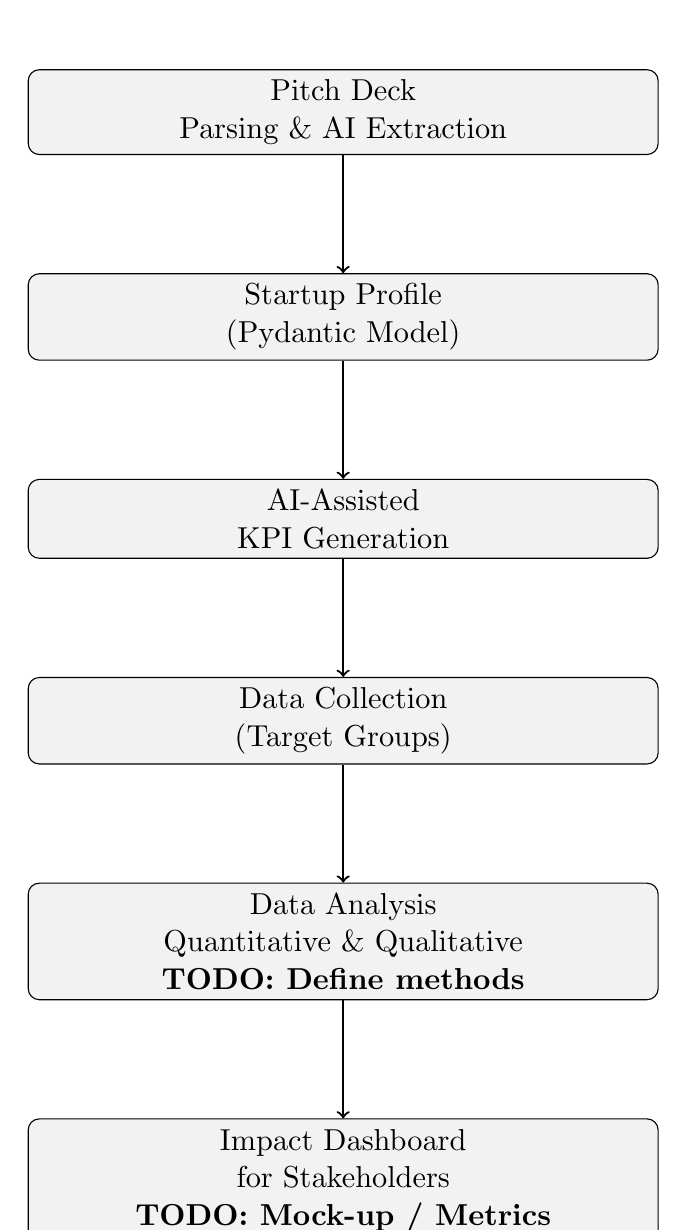
\begin{tikzpicture}[
    node distance=1.5cm,
    box/.style={rectangle, draw=black, rounded corners, fill=gray!10, minimum width=8cm, minimum height=1cm, align=center},
    arrow/.style={->, thick}
]

% Nodes
\node[box] (pitchdeck) {Pitch Deck\\Parsing \& AI Extraction};
\node[box, below=of pitchdeck] (profile) {Startup Profile\\(Pydantic Model)};
\node[box, below=of profile] (kpi) {AI-Assisted\\KPI Generation};
\node[box, below=of kpi] (data) {Data Collection\\(Target Groups)};
\node[box, below=of data] (analysis) {Data Analysis\\Quantitative \& Qualitative \\ \textbf{TODO: Define methods}};
\node[box, below=of analysis] (dashboard) {Impact Dashboard\\for Stakeholders \\ \textbf{TODO: Mock-up / Metrics}};

% Arrows
\draw[arrow] (pitchdeck) -- (profile);
\draw[arrow] (profile) -- (kpi);
\draw[arrow] (kpi) -- (data);
\draw[arrow] (data) -- (analysis);
\draw[arrow] (analysis) -- (dashboard);

\end{tikzpicture}
\caption{End-to-End Vertical Workflow: From Pitch Deck Parsing to Impact Dashboard}
\label{fig:end-to-end-pipeline-vertical}
\end{figure}

\section{Summary}\label{sec:artefact-summary}

This chapter demonstrates that the AI-supported IMM artefact can:

\begin{itemize}
    \item Efficiently onboard new projects using automated pitch deck parsing.
    \item Generate structured project profiles with AI-assisted data extraction.
    \item Produce actionable KPIs aligned with SDGs and recognized impact frameworks.
    \item Maintain a human-in-the-loop workflow for quality assurance, interpretability, and stakeholder validation.
    \item Feed collected data into a dashboard for actionable insights for impact investors.
\end{itemize}

\textbf{TODO:} Fill in the analysis methods, dashboard design, and examples before final evaluation chapter.

\chapter{Demonstration and Evaluation}\label{ch:demonstration-evaluation}

This chapter presents the \textbf{demonstration and evaluation} of the AI-supported IMM artefact developed in Chapter~\ref{ch:artefact-development}. 
The framework was tested using synthetic project data, anonymized pitch materials, and stakeholder walkthroughs, to assess its feasibility, transparency, comparability, and usability.

\section{Overview of Demonstration}\label{sec:demo-overview}

The artefact was applied in the context of \textit{Inluma} to demonstrate its functionality:

\begin{itemize}
    \item \textbf{Semantic clustering}: grouping unstructured narrative inputs into interpretable themes.
    \item \textbf{KPI derivation pipeline}: generating auditable KPIs from structured problem statements.
    \item \textbf{SDG mapping}: aligning project objectives with Sustainable Development Goals and providing transparent justifications.
\end{itemize}

The demonstration highlights the artefact's capacity to augment human judgment while remaining \textbf{transparent and interpretable}.

\section{Narrative Clustering Results}\label{sec:results-clustering}

Narratives from over 20 public innovation cases were embedded using \texttt{text-embedding-ada-002}, reduced via UMAP, and clustered with HDBSCAN.

\subsection*{Key Observations}

\begin{itemize}
    \item Clusters revealed cross-cutting themes such as citizen participation, data ethics, and local climate action.  
    \item GPT-4 summarization provided interpretable labels for stakeholders.  
    \item Clustering facilitated structured overviews of diverse inputs, supporting reflection and discussion.  
\end{itemize}

\textbf{TODO:} Include UMAP figure and example cluster summary table.

\section{SDG Mapping Results}\label{sec:results-sdg}

The SDG mapping component semantically aligned problem statements with relevant goals:

\begin{itemize}
    \item Classifier accuracy: 85\% alignment with expected SDG tags (manual benchmark).  
    \item GPT-based justifications enhanced transparency and trust.  
\end{itemize}

\textbf{Example:} 
\emph{“This project addresses SDG 11 (Sustainable Cities and Communities) by increasing civic data accessibility for participatory urban governance.”}

\textbf{TODO:} Add table with sample SDG mappings and justifications.

\section{KPI Derivation Pipeline Results}\label{sec:results-kpi}

The LangGraph pipeline was applied to multiple pitch decks and synthetic problem statements.

\subsection*{Example Output}

\begin{itemize}
    \item \textbf{Problem:} “Limited mobility access for rural elderly populations.”  
    \item \textbf{Mapped SDG:} SDG 11  
    \item \textbf{KPI:} \emph{“Percentage increase of rural elderly residents with weekly access to on-demand mobility services.”}
\end{itemize}

\subsection*{Audit Loop Observations}

\begin{itemize}
    \item KPIs with quality scores below 80\% were regenerated in 42\% of test runs.  
    \item Common issues: vague definitions, misalignment with outcomes.  
    \item Audit loops proved essential for maintaining consistency and alignment.  
\end{itemize}

\textbf{TODO:} Include pipeline flow diagram and example output tables.

\section{Human-in-the-Loop Feedback}\label{sec:results-hitl}

Stakeholder walkthroughs confirmed the importance of \textbf{human validation}:

\begin{itemize}
    \item Manual editing of AI-generated problem statements was often needed.  
    \item Feedback loops validated SDG and KPI proposals.  
    \item Alternative perspectives were incorporated through iterative discussion.  
\end{itemize}

This reinforces the artefact’s design principle: AI as a \textbf{decision-support tool}, not a replacement for human expertise.

\section{Transparency and Explainability}\label{sec:results-xai}

Each pipeline run logged \textbf{decision paths and rationales}, supporting audits and ethical review:

\begin{itemize}
    \item Justifications captured at SDG mapping, indicator selection, and KPI generation.  
    \item SHAP and GPT-based explanations provided interpretable insights.  
    \item Supports accountability and trust in AI-supported evaluation processes.  
\end{itemize}

\textbf{TODO:} Include example trace schematic.

\section{Evaluation Summary}\label{sec:results-summary}

The artefact was evaluated against pre-defined DSR criteria:

\begin{itemize}
    \item \textbf{Feasibility:} All modules operated successfully on test datasets.  
    \item \textbf{Transparency:} Justifications and audit loops increased interpretability.  
    \item \textbf{Comparability:} Semantic clustering and KPI derivation facilitated consistent evaluation across cases.  
    \item \textbf{Usability:} Stakeholders found outputs informative, with manageable human-in-the-loop requirements.  
\end{itemize}

\textbf{Key insights:}  

\begin{itemize}
    \item AI tools can support reflective, value-aligned impact assessment.  
    \item Human-in-the-loop mechanisms are essential for interpretability and trust.  
    \item Modular design allows adaptation to different data sources and contexts.  
\end{itemize}

The next chapter discusses these results in the context of existing frameworks, reflecting on theoretical and practical implications.

%! Author = deandidion
%! Date = 09.07.25

% Preamble
\chapter{Conclusion}
\section{Summary}
\lipsum[15]
\section{Future Work}
\lipsum[16]



\nocite{*}
\printbibliography

\clearpage

\appendix

%! Author = deandidion
%! Date = 11.07.25

\chapter{Additional Data}\label{ch:additional-data}

This appendix contains supplementary data and materials that support the findings and analyses presented in the main chapters of the thesis.

\section*{Data Tables}



\vspace{2em}

\section*{Additional Figures}



\vspace{2em}

\section*{Raw Data Excerpts}

\noindent Below are anonymized excerpts from the interview transcripts used for qualitative analysis:

\begin{quote}
    \textit{"One of the biggest barriers is trust — people often question how AI reaches its conclusions."}
\end{quote}

\begin{quote}
    \textit{"Having a clear framework aligned with public values ensures the tool's relevance and acceptance."}
\end{quote}

\vspace{2em}

% You can add more tables, fig, or text here as needed.

\end{document}
o